\documentclass{standalone}
\usepackage{tikz}
\usetikzlibrary{patterns, positioning}


\begin{document}
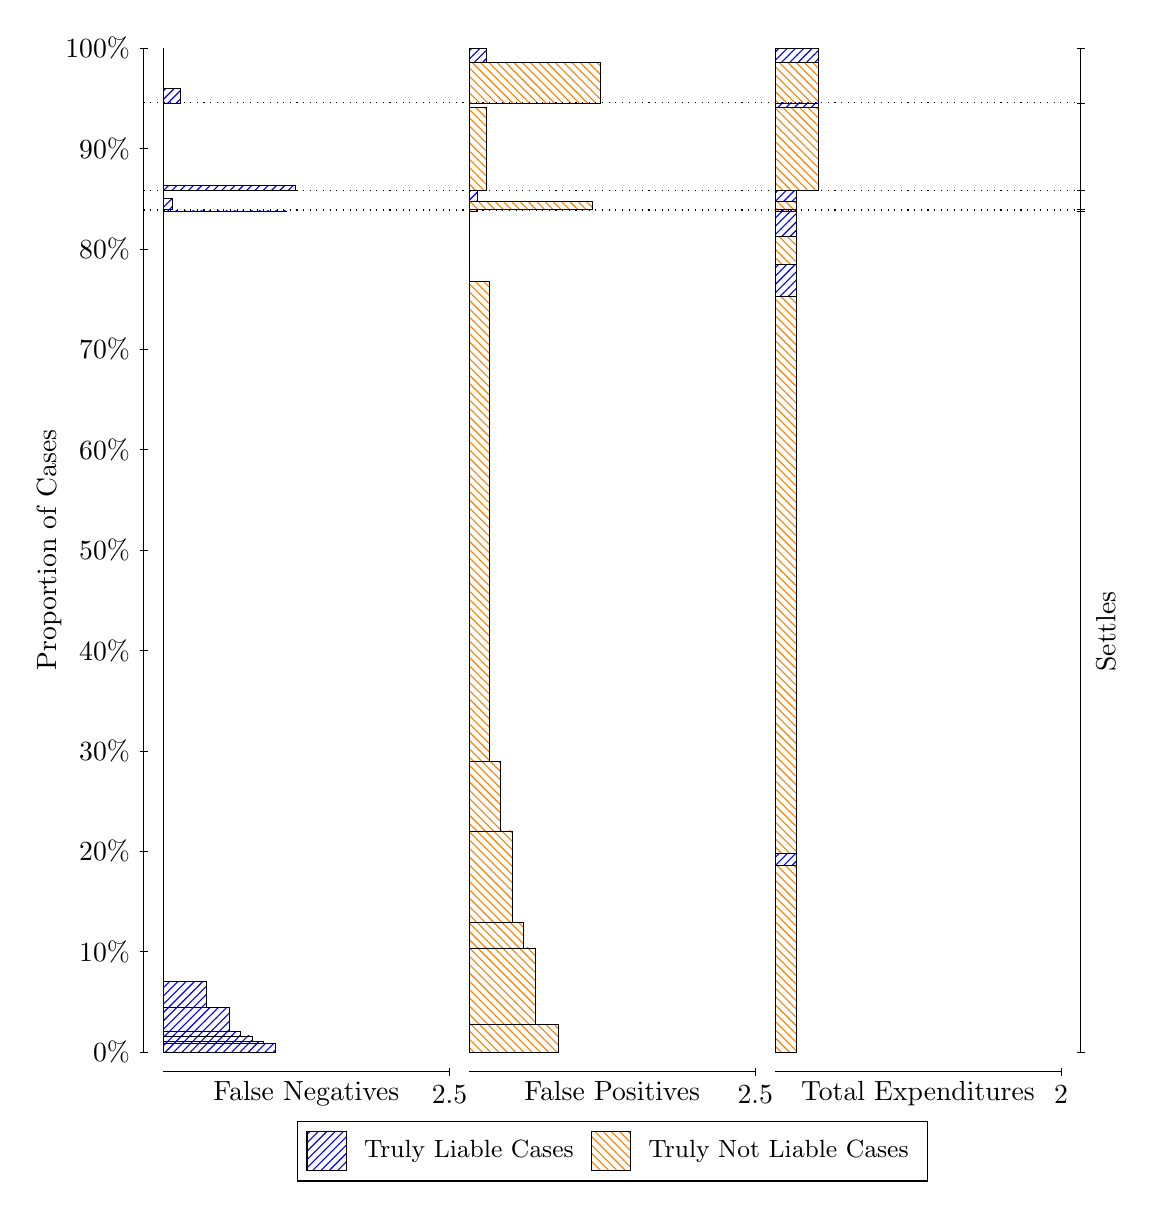
\begin{tikzpicture}
\draw[black, very thin] (1.5,1.75) -- (1.5,14.5);
\node[rotate=90, text=black, anchor=center] at (0.3, 8.125) {Proportion of Cases};
\draw[black, very thin] (1.45,1.75) -- (1.55,1.75);
\node[text=black, anchor=east] at (1.45, 1.75) {0\%};
\draw[black, very thin] (1.45,3.025) -- (1.55,3.025);
\node[text=black, anchor=east] at (1.45, 3.025) {10\%};
\draw[black, very thin] (1.45,4.3) -- (1.55,4.3);
\node[text=black, anchor=east] at (1.45, 4.3) {20\%};
\draw[black, very thin] (1.45,5.575) -- (1.55,5.575);
\node[text=black, anchor=east] at (1.45, 5.575) {30\%};
\draw[black, very thin] (1.45,6.85) -- (1.55,6.85);
\node[text=black, anchor=east] at (1.45, 6.85) {40\%};
\draw[black, very thin] (1.45,8.125) -- (1.55,8.125);
\node[text=black, anchor=east] at (1.45, 8.125) {50\%};
\draw[black, very thin] (1.45,9.4) -- (1.55,9.4);
\node[text=black, anchor=east] at (1.45, 9.4) {60\%};
\draw[black, very thin] (1.45,10.675) -- (1.55,10.675);
\node[text=black, anchor=east] at (1.45, 10.675) {70\%};
\draw[black, very thin] (1.45,11.95) -- (1.55,11.95);
\node[text=black, anchor=east] at (1.45, 11.95) {80\%};
\draw[black, very thin] (1.45,13.225) -- (1.55,13.225);
\node[text=black, anchor=east] at (1.45, 13.225) {90\%};
\draw[black, very thin] (1.45,14.5) -- (1.55,14.5);
\node[text=black, anchor=east] at (1.45, 14.5) {100\%};

\draw[black, very thin] (13.4,1.75) -- (13.4,14.5);
\draw[black, very thin] (13.35,1.75) -- (13.45,1.75);
\node[anchor=west] at (13.35, 1.75) {};
\draw[black, very thin] (13.35,12.432) -- (13.45,12.432);
\node[anchor=west] at (13.35, 12.432) {};
\draw[black, very thin] (13.35,12.449) -- (13.45,12.449);
\node[anchor=west] at (13.35, 12.449) {};
\draw[black, very thin] (13.35,12.694) -- (13.45,12.694);
\node[anchor=west] at (13.35, 12.694) {};
\draw[black, very thin] (13.35,13.804) -- (13.45,13.804);
\node[anchor=west] at (13.35, 13.804) {};
\draw[black, very thin] (13.35,14.5) -- (13.45,14.5);
\node[anchor=west] at (13.35, 14.5) {};

\draw[black, very thin, pattern color=blue, pattern=north east lines] (1.75,1.75) rectangle (3.167,1.8596);
\draw[black, very thin, pattern color=blue, pattern=north east lines] (1.75,1.8596) rectangle (3.0217,1.882);
\draw[black, very thin, pattern color=blue, pattern=north east lines] (1.75,1.882) rectangle (2.8763,1.9556);
\draw[black, very thin, pattern color=blue, pattern=north east lines] (1.75,1.9556) rectangle (2.731,2.0146);
\draw[black, very thin, pattern color=blue, pattern=north east lines] (1.75,2.0146) rectangle (2.5857,2.3204);
\draw[black, very thin, pattern color=blue, pattern=north east lines] (1.75,2.3204) rectangle (2.295,2.6467);
\draw[black, very thin, pattern color=orange, pattern=north west lines] (1.75,2.6467) rectangle (1.75,12.432);
\draw[black, very thin, pattern color=blue, pattern=north east lines] (1.75,12.432) rectangle (3.3123,12.433);
\draw[black, very thin, pattern color=orange, pattern=north west lines] (1.75,12.433) rectangle (1.75,12.449);
\draw[black, very thin, pattern color=blue, pattern=north east lines] (1.75,12.449) rectangle (1.859,12.59);
\draw[black, very thin, pattern color=orange, pattern=north west lines] (1.75,12.59) rectangle (1.75,12.694);
\draw[black, very thin, pattern color=blue, pattern=north east lines] (1.75,12.694) rectangle (3.4213,12.751);
\draw[black, very thin, pattern color=orange, pattern=north west lines] (1.75,12.751) rectangle (1.75,13.804);
\draw[black, very thin, pattern color=blue, pattern=north east lines] (1.75,13.804) rectangle (1.968,13.984);
\draw[black, very thin, pattern color=orange, pattern=north west lines] (1.75,13.984) rectangle (1.75,14.5);
\draw[black, very thin, pattern color=orange, pattern=north west lines] (5.6333,1.75) rectangle (6.7597,2.0999);
\draw[black, very thin, pattern color=orange, pattern=north west lines] (5.6333,2.0999) rectangle (6.469,3.0729);
\draw[black, very thin, pattern color=orange, pattern=north west lines] (5.6333,3.0729) rectangle (6.3237,3.3991);
\draw[black, very thin, pattern color=orange, pattern=north west lines] (5.6333,3.3991) rectangle (6.1783,4.5565);
\draw[black, very thin, pattern color=orange, pattern=north west lines] (5.6333,4.5565) rectangle (6.033,5.4437);
\draw[black, very thin, pattern color=orange, pattern=north west lines] (5.6333,5.4437) rectangle (5.8877,11.536);
\draw[black, very thin, pattern color=blue, pattern=north east lines] (5.6333,11.536) rectangle (5.6333,12.432);
\draw[black, very thin, pattern color=orange, pattern=north west lines] (5.6333,12.432) rectangle (5.7423,12.449);
\draw[black, very thin, pattern color=blue, pattern=north east lines] (5.6333,12.449) rectangle (5.6333,12.449);
\draw[black, very thin, pattern color=orange, pattern=north west lines] (5.6333,12.449) rectangle (7.1957,12.553);
\draw[black, very thin, pattern color=blue, pattern=north east lines] (5.6333,12.553) rectangle (5.7423,12.694);
\draw[black, very thin, pattern color=orange, pattern=north west lines] (5.6333,12.694) rectangle (5.8513,13.747);
\draw[black, very thin, pattern color=blue, pattern=north east lines] (5.6333,13.747) rectangle (5.6333,13.804);
\draw[black, very thin, pattern color=orange, pattern=north west lines] (5.6333,13.804) rectangle (7.3047,14.32);
\draw[black, very thin, pattern color=blue, pattern=north east lines] (5.6333,14.32) rectangle (5.8513,14.5);
\draw[black, very thin, pattern color=orange, pattern=north west lines] (9.5167,1.75) rectangle (9.7892,4.1208);
\draw[black, very thin, pattern color=blue, pattern=north east lines] (9.5167,4.1208) rectangle (9.7892,4.2758);
\draw[black, very thin, pattern color=orange, pattern=north west lines] (9.5167,4.2758) rectangle (9.7892,11.341);
\draw[black, very thin, pattern color=blue, pattern=north east lines] (9.5167,11.341) rectangle (9.7892,11.756);
\draw[black, very thin, pattern color=orange, pattern=north west lines] (9.5167,11.756) rectangle (9.7892,12.106);
\draw[black, very thin, pattern color=blue, pattern=north east lines] (9.5167,12.106) rectangle (9.7892,12.432);
\draw[black, very thin, pattern color=orange, pattern=north west lines] (9.5167,12.432) rectangle (9.7892,12.449);
\draw[black, very thin, pattern color=blue, pattern=north east lines] (9.5167,12.449) rectangle (9.7892,12.449);
\draw[black, very thin, pattern color=orange, pattern=north west lines] (9.5167,12.449) rectangle (9.7892,12.553);
\draw[black, very thin, pattern color=blue, pattern=north east lines] (9.5167,12.553) rectangle (9.7892,12.694);
\draw[black, very thin, pattern color=orange, pattern=north west lines] (9.5167,12.694) rectangle (10.062,13.747);
\draw[black, very thin, pattern color=blue, pattern=north east lines] (9.5167,13.747) rectangle (10.062,13.804);
\draw[black, very thin, pattern color=orange, pattern=north west lines] (9.5167,13.804) rectangle (10.062,14.32);
\draw[black, very thin, pattern color=blue, pattern=north east lines] (9.5167,14.32) rectangle (10.062,14.5);
\draw[black, dotted] (1.5,12.432) -- (13.4,12.432);
\draw[black, dotted] (1.5,12.449) -- (13.4,12.449);
\draw[black, dotted] (1.5,12.694) -- (13.4,12.694);
\draw[black, dotted] (1.5,13.804) -- (13.4,13.804);
\draw[black, very thin] (1.75,1.5) -- (5.3833,1.5);
\node[text=black, anchor=north] at (3.5667, 1.5) {False Negatives};
\draw[black, very thin] (5.3833,1.45) -- (5.3833,1.55);
\node[text=black, anchor=north] at (5.3833, 1.45) {2.5};

\draw[black, very thin] (5.6333,1.5) -- (9.2667,1.5);
\node[text=black, anchor=north] at (7.45, 1.5) {False Positives};
\draw[black, very thin] (9.2667,1.45) -- (9.2667,1.55);
\node[text=black, anchor=north] at (9.2667, 1.45) {2.5};

\draw[black, very thin] (9.5167,1.5) -- (13.15,1.5);
\node[text=black, anchor=north] at (11.333, 1.5) {Total Expenditures};
\draw[black, very thin] (13.15,1.45) -- (13.15,1.55);
\node[text=black, anchor=north] at (13.15, 1.45) {2};

\node[text=black, centered, rotate=90] at (13.72, 7.0912) {Settles};





\draw (7.449999999999999,1.5) node[draw=none] (baseCoordinate) {};
\begin{scope}[align=center]
        \matrix[scale=0.5, draw=black, below=0.5cm of baseCoordinate, nodes={draw}, column sep=0.1cm]{
            \node[rectangle, draw, minimum width=0.5cm, minimum height=0.5cm, pattern color=blue, pattern=north east lines] {}; &
            \node[draw=none, font=\small, text=black] (B) {Truly Liable Cases}; &
            \node[rectangle, draw, minimum width=0.5cm, minimum height=0.5cm, pattern color=orange, pattern=north west lines] {}; &
            \node[draw=none, font=\small, text=black] (B) {Truly Not Liable Cases}; \\
            };
\end{scope}

\end{tikzpicture}
\end{document}